% Chapter 4it

\begin{savequote}[\quotewidth]
$pV \neq nRT$ 
\qauthor{The universal gas law does not apply to supercritical fluids}
\end{savequote}

\chapter{Instrumentation: Supercritical Fluid Chromatography} % Main chapter title

\label{Chapter4} % For referencing this chapter elsewhere, use \ref{Chapter4}

This thesis discusses the development of a comprehensively coupled
(supercritical fluid × gas) chromatograph and its application to the analysis of
biodiesel. The discussion on the experimental work divides naturally into two
parts: this chapter discusses the supercritical fluid chromatography (SFC) and
the next chapter discusses the gas chromatography (GC).

\section{SFC}

As discussed in Chapter \ref{Chapter2}, an SFC chromatograph consists of a
supply of mobile phase, a pump, a pressure control system, a modifier control
system, a column, a pressure relief system and a detector

\section{Mobile phase}

As mobile phase we used carbon dioxide. The benefits of carbon dioxide as an
solvent and mobile phase is discussed in Chapter \ref{Chapter2}.

We used 99.995 \% pure carbon dioxide supplied by Air Produts. Our colleauges in
industry also use food grade or technical grade carbon dioxide and they have
not reported any significant impurities.

As modifier we used LiChrosolv\textregistered methanol from Merck. This is an
`HPLC-grade' solvent, of which the purification is optimized for the removal of
UV-absorbing impurities. Using this grade of solvents is important when using
optical aborbance or fluorescence detectors, because lowering levels of
impurities improve limits of detection. It is quite likely that a less expensive
grade of modifier would also be suitable for our SFC, because we do not use an
optical detector.

\section{Pump}
\label{sec:CO2Pump}

As pump we used the robust, reliable Varian 8500 HPLC pump because it was
available. This pump had its control electronics removed, and it was controlled
from a personal computer by software written for the purpose.

The Varian 8500 pump is driven by a stepper motor. This kind of motor turns in
discrete steps, instead of at a constant rate. It is driven by pulses of
electric current, rather than a continuous current, and therefore the speed of
the motor can be controlled by varying the rate of the pulses. This makes it
relatively simple to control the speed of the motor from a computer.

The Varian 8500 pump has a built-in pressure transducer that provided an
electronic signal proportional to the pressure at the pump outlet.

The Varian 8500 pump is a single-piston pump with a 250 \si{\milli\litre} capacity that
needs to be refilled between strokes. Refilling means that one has to stop
chromatography, which makes it important to fill the pump to full capacity, so
that chromatographic runs are not interrupted. This means that the pump needs to
be filled with carbon dioxide in the liquid phase rather than the vapour phase.
Compressing either would create the appropriate phase for doing chromatography,
but compressing a vapour would leave one with a much smaller volume of
high-pressure carbon dioxide than compressing a liquid.

Filling a pump with liquid carbon dioxide is more difficult than one might
imagine. 


\begin{figure}
\centering
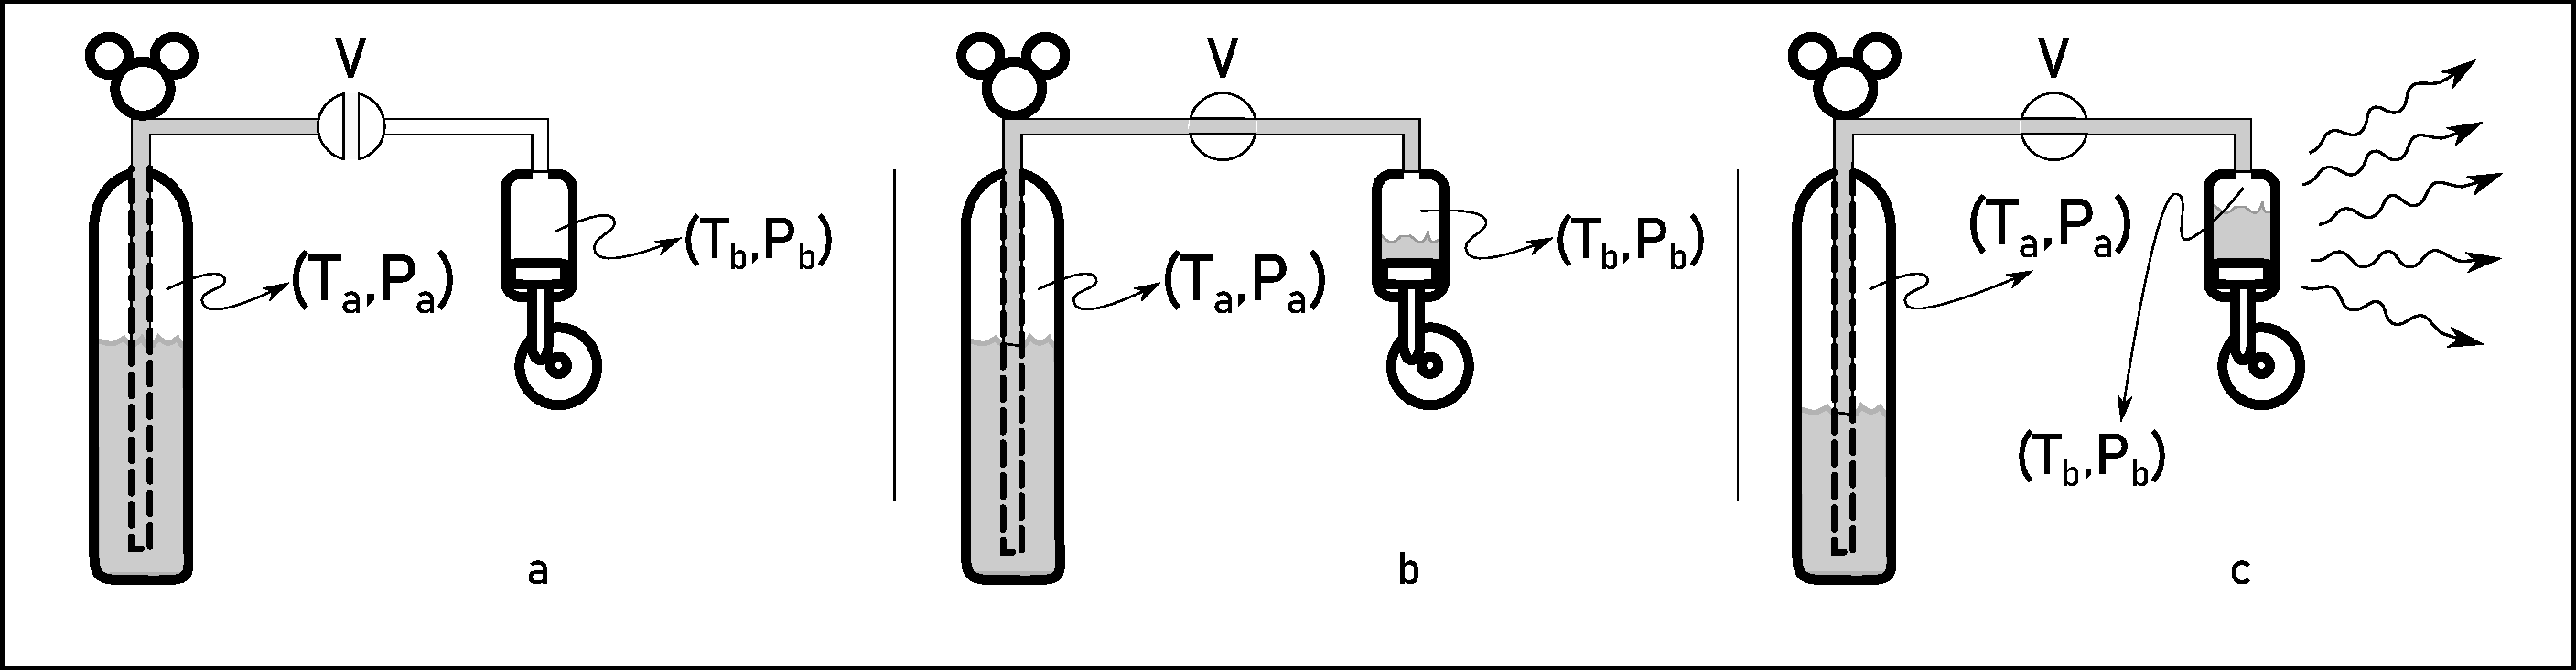
\includegraphics[width=\textwidth]{Figures/CO2Filling.pdf}
\decoRule

\caption[Fillng a CO\textsubscript{2} pump.]{Diagram to help explain the filling of
the carbon dioxide pump. (a) The pressure in the reservoir $P_a$ is much higher
than the pressure in the receptacle $P_b$. The valve is closed, so there is no
flow. (b) The valve is open and some carbon dioxide has flowed from the
reservoir to the receptacle. But $P_b = P_a$, so there is no flow. (c) When the
temperature in the receptacle $T_b < T_a$, then $P_b  < P_a$, following
Gay-Lussac's law. Flow will continue until all the vapour in the receptacle has
condensed.}

\label{fig:co2fill}
\end{figure}


Imagine a reservoir of liquid carbon dioxide, equipped with a dip tube,
connected to an empty receptacle via a valve (V). (See Figure \ref{fig:co2fill})
One can assume that the receptacle is empty and contains only carbon dioxide
vapour at atmospheric pressure, say 1 atm. The vapour pressure of the vapour
above the liquid in the reservoir is about 55.3 atm (5.6 MPa).
When the valve (V) is opened the will high-pressure vapour in the reservoir will
expel the liquid carbon dioxide through the dip tube and through the valve, into
the receptacle. In the low-pressure environment of the receptacle the carbon
dioxide will boil. Soon there will be some liquid carbon dioxide in the
receptacle, with the rest of the receptacle volume filled with gaseous carbon
dioxide. When the system comes to equilibrium the pressure in the receptacle
($P_b$) will equal the pressure in the reservoir ($P_a$), and there will be no
flow of liquid carbon dioxide. One can attempt to now increase the flow by
increasing the volume of the receptacle (for example by withdrawing a pump
piston), and hence decreasing the vapour pressure there.
But any flow from the reservoir will lead to expansion of the headspace of the
reservoir. This will lead to cooling of the vapour, and therefore lower pressure
and therefore lower flow. The final result of this process is that the
receptacle is never filled to capacity with liquid.

The only way to restore the flow from the reservoir to the recepacle is to
create a pressure difference $P_a - P_b$. While it is possible to create an
overpressure in the reservoir by adding a headspace gas, it is technically
challenging and expensive. It is simpler to use the Guy-Lussac gas law.
According to this law the ratio of the pressure to the temperature of a gas is
constant so that $\frac{P_b}{T_b} = k$. This means that a decrease in
temperature will lead to a decrease in pressure. The way to fill the reservoir
to capacity is to ensure that the temperature of headspace vapour $T_a$ is higher
than the temperature of the headspace vapour $T_b$. Because safety regulations
prohibit the heating of a cylinder of pressurized gas, the way to ensure $T_a <
T_b$ is to cool the receptacle. This cools the headspace vapour, and following
the Gay-Lussac law the pressure $P_b$ decreases, the difference $P_a - P_b$
increases and the liquid flows until the receptacle is filled to capacity.
 
In the case of the Varian 8500 pump the cooling of the pump was achieved by
wrapping a coil of copper tubing around the cylinder, and pumping a chilled
heat-exchange fluid through it. A chiller with a mechanically cooled tank with a
20 l capacity was filled with a solution of 5.0 l of diethyl glycerol in about
10 l of water. This mixture has a freezing point of -15 \si{\degreeCelsius},
which can be cooled by the chiller without freezing. (If the coolant freezes a
layer of ice forms on the cooling plate of the chiller, which isolates the
remaining liquid from the cooling plate and limits the minimum temperature of
the coolant.) An inexpensive submersible water pump (designed for decorative
water fountains) was used to pump the coolant through the circuit.
This pump can deliver 800 l of water per hour at a head of 1.2 \si{\metre}.

For some experiments we also used a SFT-10 pump from Supercritical Fluid
Technologies (Newark, Delaware). This is a purpose-built two-piston pump with a
sapphire valve seats and a Peltier-cooled head. This is a much better technology
than the HPLC pumps. It takes up less space and does not need refilling, since
it feeds directly from the cylinder. This pump had its own microprocessor
controllers on board, and flow and pressure could simply be commanded from the
PC through a USB cable.

\subsection{Pressure control system}

The aim of chromatography is to separate chromatograms by a certain distance.
But the days of separating coloured compounds in glass packed columns are long
past and the direct measurement of distances are now relegated to thin-layer
chromatography. Instead, we have to make do with proxies for distance such as \textit{retention
volumes} or \textit{retention times}. 


% In chromatography the figure of merit by which the performance of a system is
% measured is the distance by which two compounds are separated, relative to their peak
% widths. This is known as the \textit{resolution}. 

Retention times are particularly convenient today, because it can easily be
measured by computer systems.

Retention times, however, depend on a known flow rate of the mobile phase
through the column. The flow rate need not be constant, although for the sake of
simplicity a constant flow rate is preferred. Ideally, the flow rate should also be
adjustable.

The need for an adjustable, constant flow rate can be met by using a control
system. Control systems are well understood by engineers, among whom it is a
major field of study \autocite{Koenig2009}. 

Figure \ref{fig:processcontrol} shows a diagram of a simple process control
system. Some aspect of the process under control is measured, which yields the
\textit{process variable} (PV). The PV is compared to the \textit{set value}
(SV), and the \textit{error} (e) is obtained by finding the difference. The error
is provided to the controller, which calculates the \textit{manipulated
variable} (MV). The MV is used to drive the final control element, which adjusts
the process with the aim of producing a smaller error.

\begin{figure}
\centering
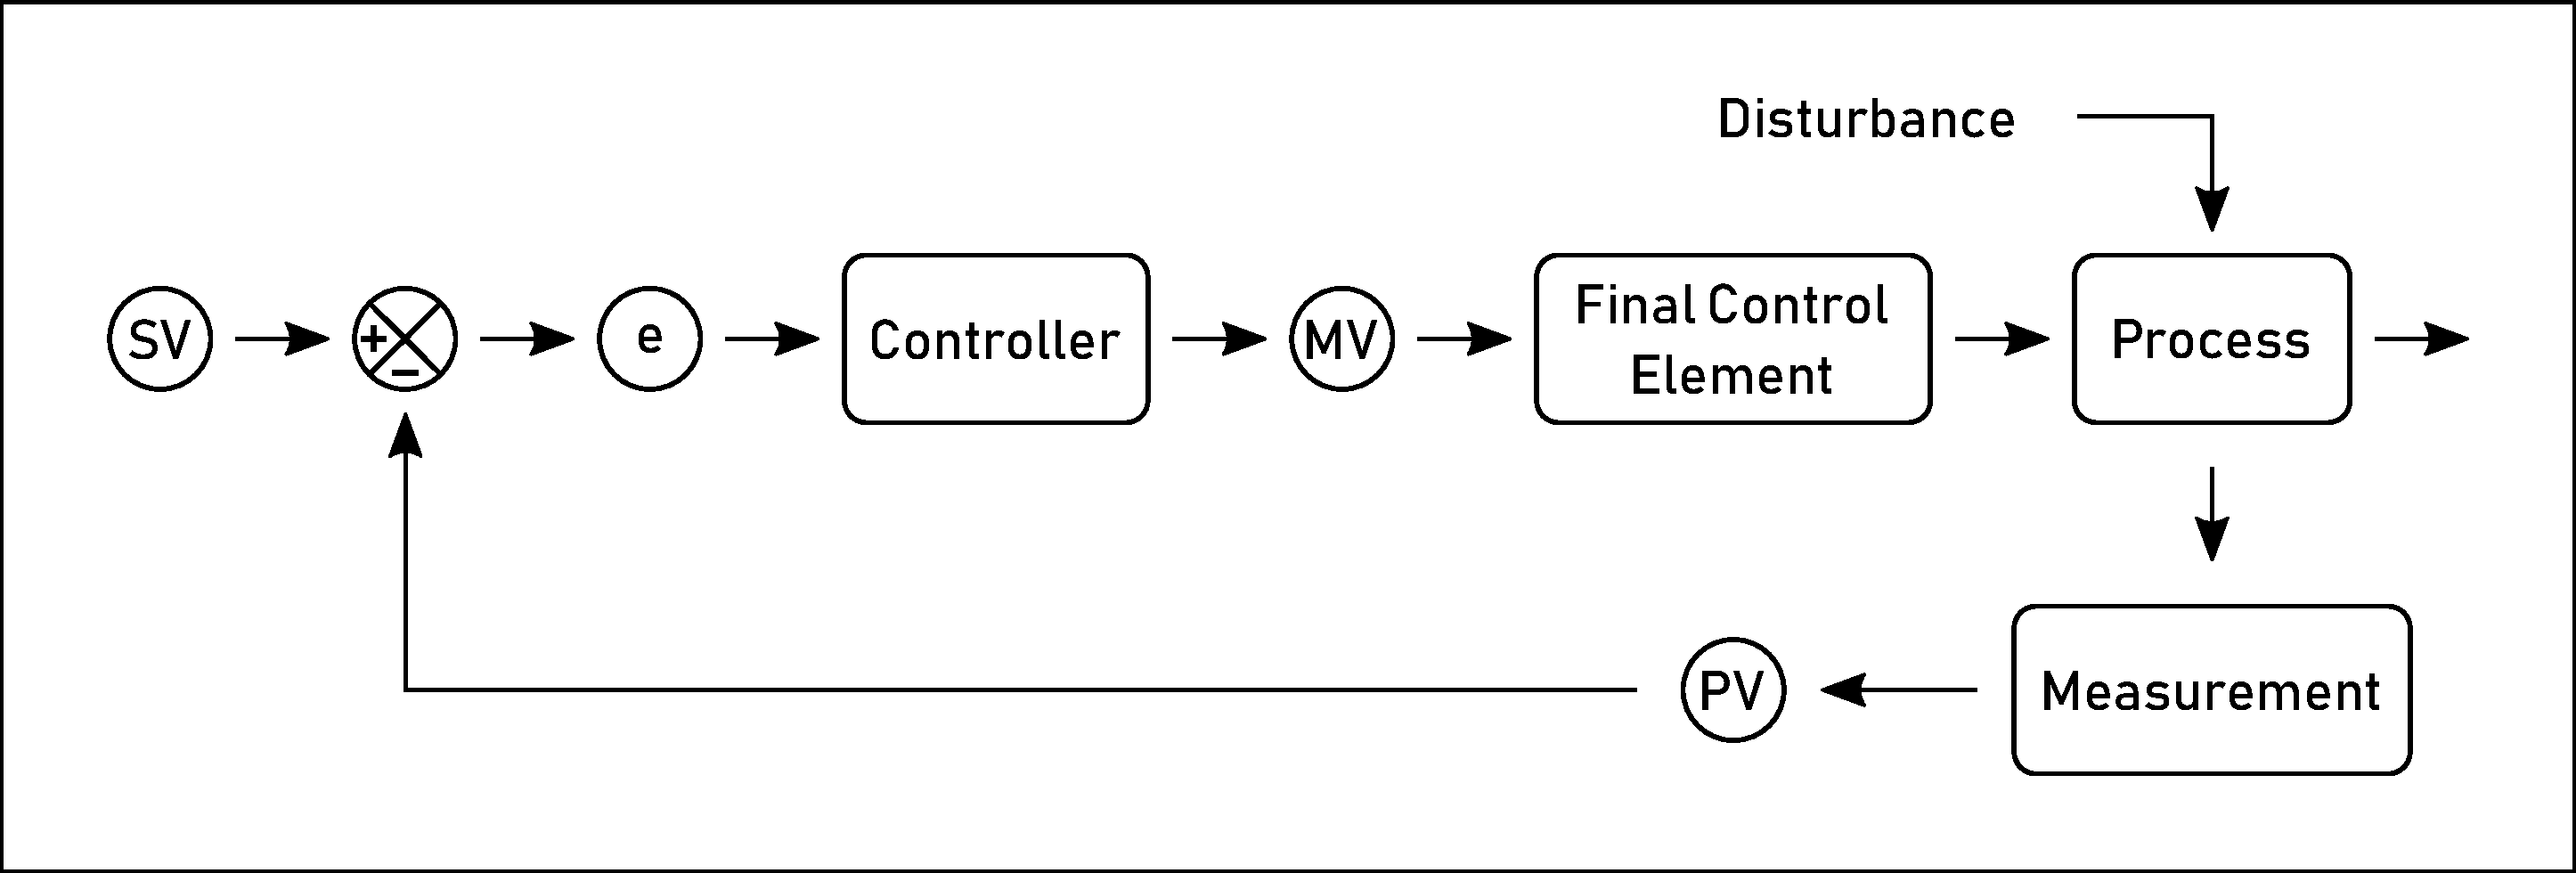
\includegraphics[width=\textwidth]{Figures/ProcessControl.pdf}
\decoRule

\caption[A process control system]{Schematic diagram of a closed-loop control
system. (SV) Set Value, (PV) Process Variable, (e) Error, (MV) Manipulated
Variable}

\label{fig:processcontrol}
\end{figure}

Chromatographic systems conventionally work under pressure control or flow
control regimes. Either is suitable: constant pressure systems usually yield
constant flow if other parameters are held constant. Because flow measurement is
more complex than pressure measurement, pressure control is the older, simpler
and less expensive control method. Also, in SFC the solvent strength of the mobile
phase is pressure/density dependent. We therefore selected pressure control
as our control regime.

In our system the pressure measured by the on-pump sensor was the process
variable (PV) . This was compared to the set value (SV) set on the computer
console. The controller was a software algorithm, implemented as a virtual
instrument in the programming environment LabVIEW. The controller computed an
output value for the manipulated variable (MV), which was the rate at which
pulses were sent to the pump, in hertz. The digital input/output (DIO) interface
of a National Instruments PCI-6014 multifunction data acquisition board created
those pulses and sent them to the pump's electronic interface.

The software used a PID (Proportional-Integral-Derivative) controller module,
with the Integral and Derivative contributions disabled. The simpler
proportional control was found totally adequate for our purpose, and it can be
improved in future by finding an appropriate tuning method and applying it with
the integral and/or derivative activated.

% While enabling the Integral and Derivative contributions would add to the
% accuracy of the controller, we could not find a suitable, simple tuning
% procedure.

% Tuning the controller from adequate performance to optimum performance would
% consume resources while not improving the chromatography.

\subsection{Modifier Control}

The modifier needs to be present in the mobile phase at a known and controlled
concentration.

There are various SFC-modifier mobile phase supply units on the market. They
tend to be a expensive and complex, because they require the use of two
controlled, high-pressure pumps. Given that our needs were rather modest, we
elected to use a simpler system.

Instead of accurately pumping the supercritical fluid and the modifier, we only
pump and control the supercritical carbon dioxide and add measured volumes of
modifier.

The modifier control unit consisted of a six-port valve, a fixed-volume
measuring loop, and a mixing chamber. 

The unit operates by filling the measuring loop with modifier, and then
switching the measuring loop into the flowing mobile phase. The modifier is
washed into the mixing chamber, where it is intimately mixed with and dissolved
in the supercritical carbon dioxide. The concentration of modifier in the mobile
phase is determined by the switching rate of the sampling valve. Given that
about 3 volumes of supercritical carbon dioxide is needed to wash the modifier
out of the loop, the highest concentration of modifier that can be added in this
manner is about 25 \%.

Figure \ref{fig:mixingchamber} shows the chosen design of the mixing chamber.
The inlet and outlet pipes of the mixing chamber extend far into the chamber, to
break up plug flow and encourage rapid mixing.  

\begin{figure}
\centering
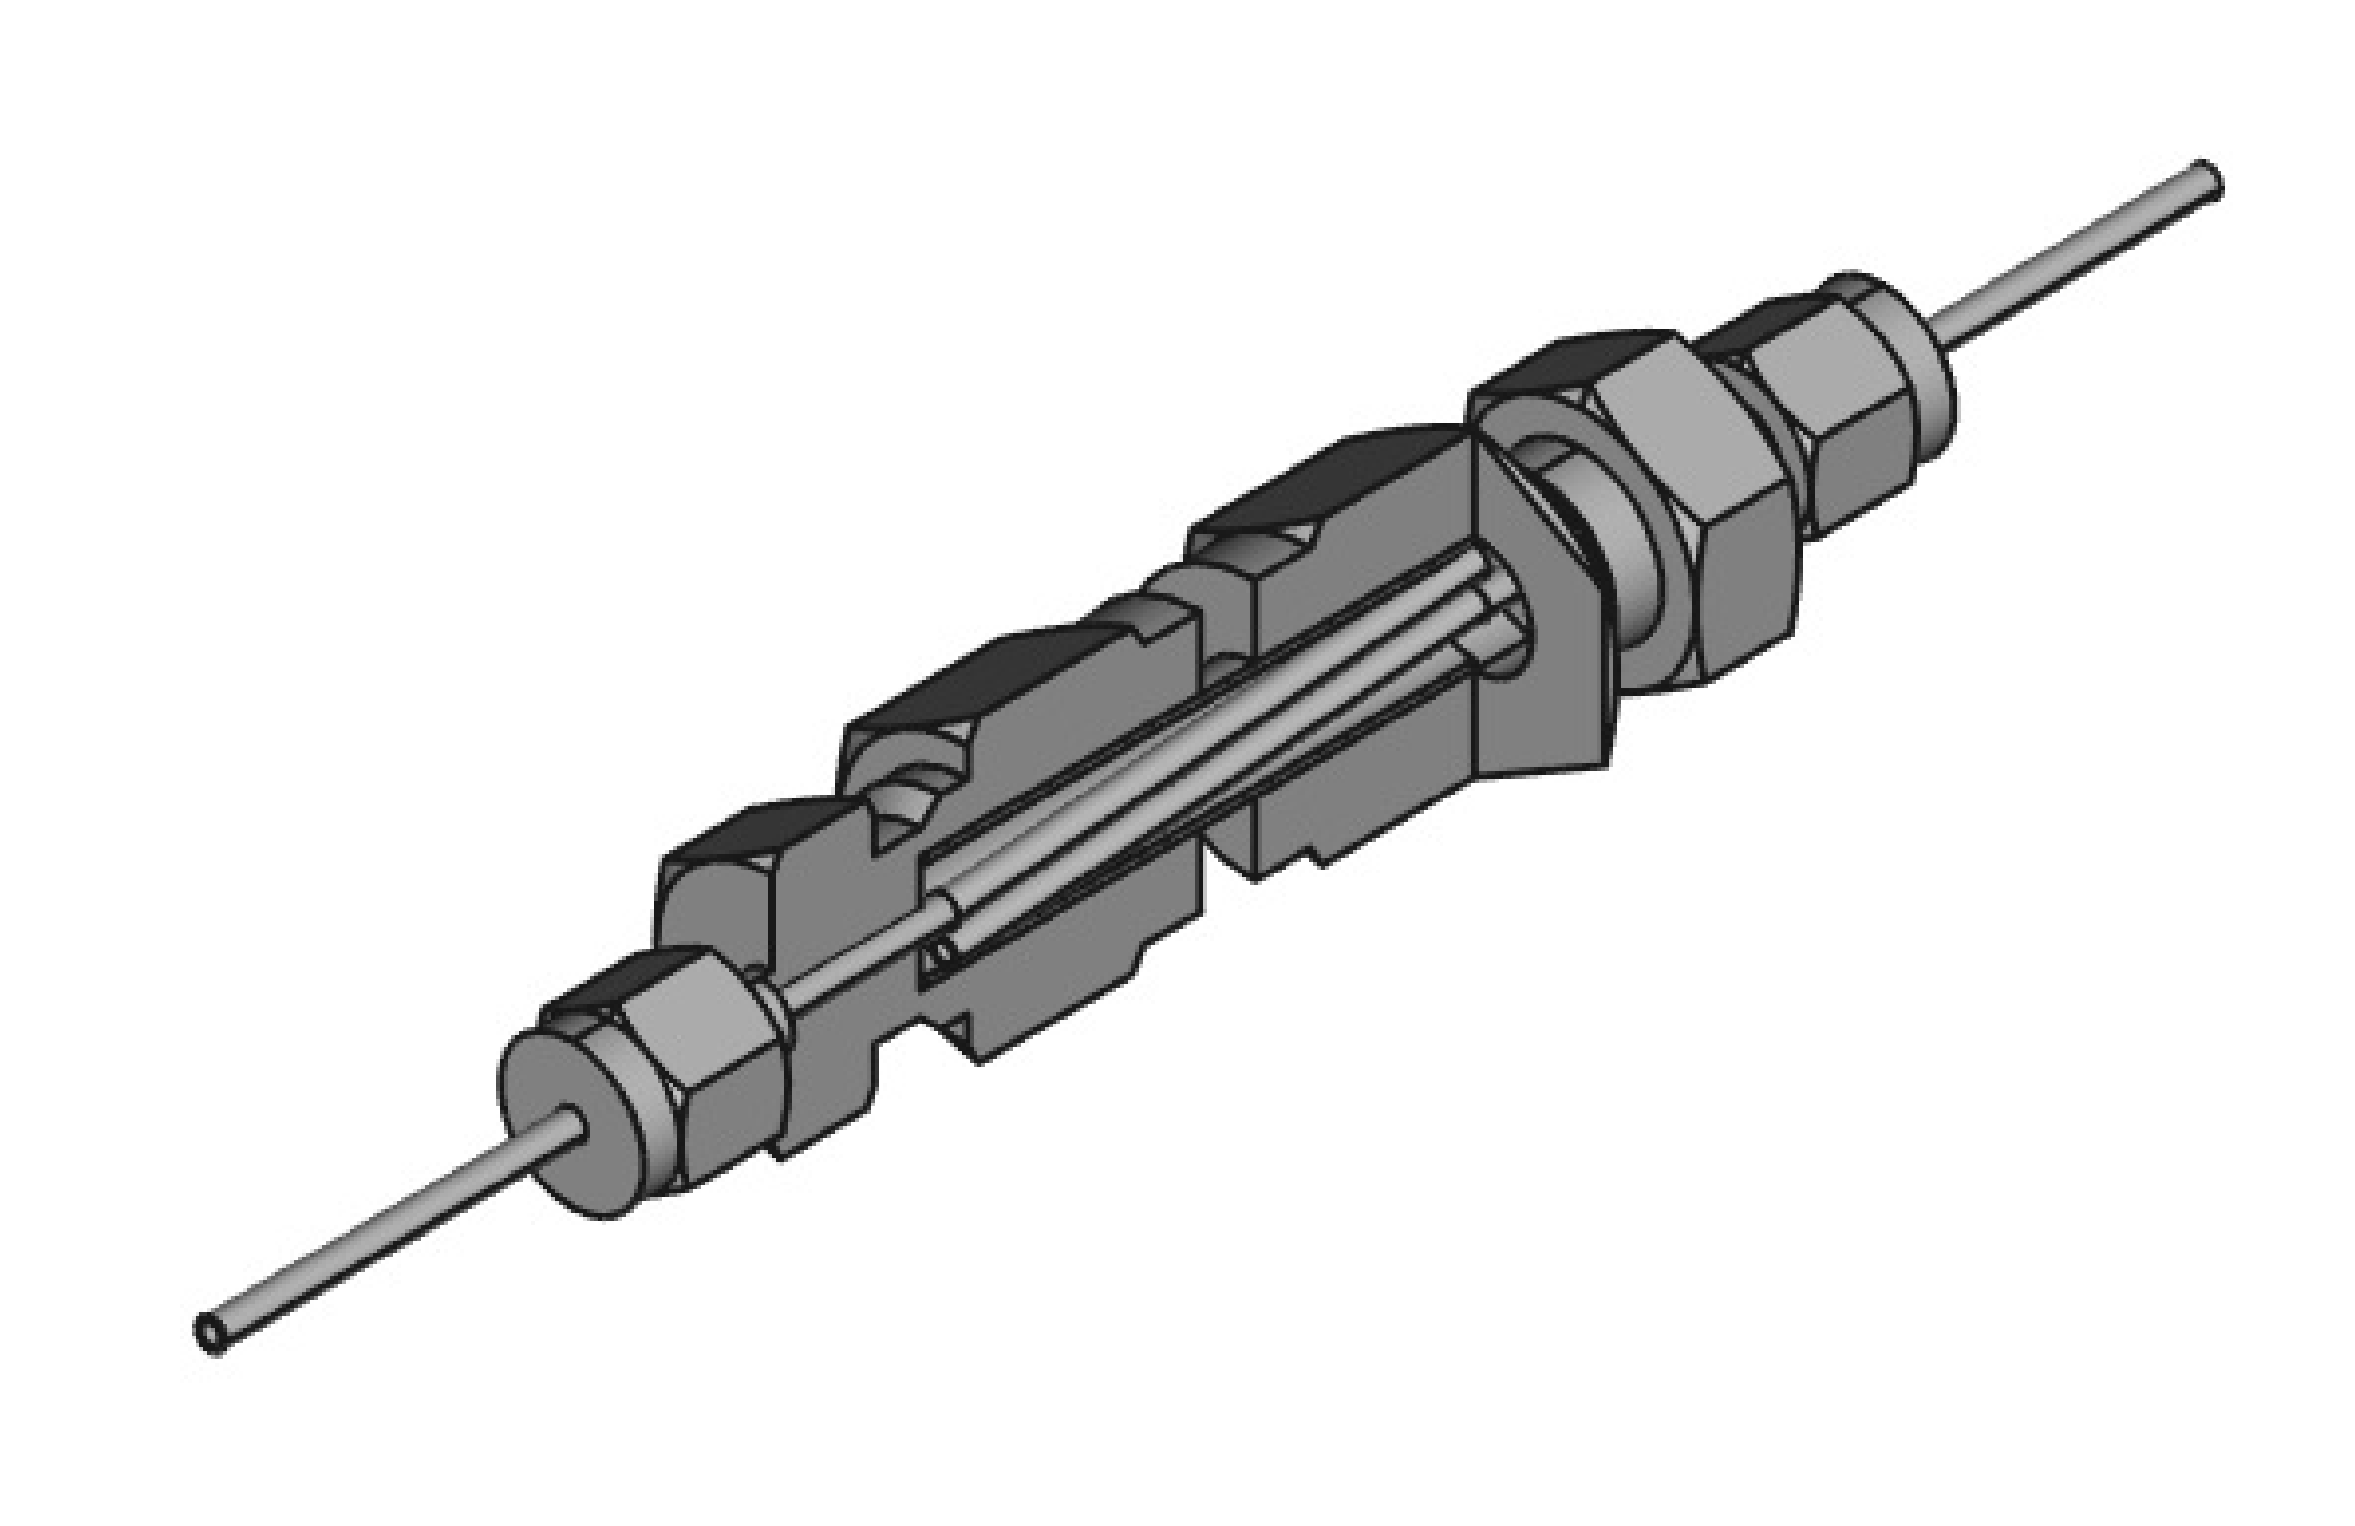
\includegraphics[width=\textwidth]{Figures/MixingChamber.png}
\decoRule

\caption[A cutaway diagram of the mixing chamber]{A cutaway diagram of the
mixing chamber design. The chamber is designed for the mixing of the modifier
and the supercritical carbon dioxide.}

\label{fig:mixingchamber}
\end{figure}

The modifier injection valve position was commanded from the controlling PC by electronic
voltage pulses.

\section{Sample injection}
\label{sec:SFCInjection}

The sample inlet was a two-position rotary valve with an internal sampling volume
(Figure \ref{fig:samplingvalve}). In one position the sampling volume was filled
with a syringe, and when the valve was commanded to inject the sampling volume
was switched into the carrier mobile stream.

\begin{figure}
\centering
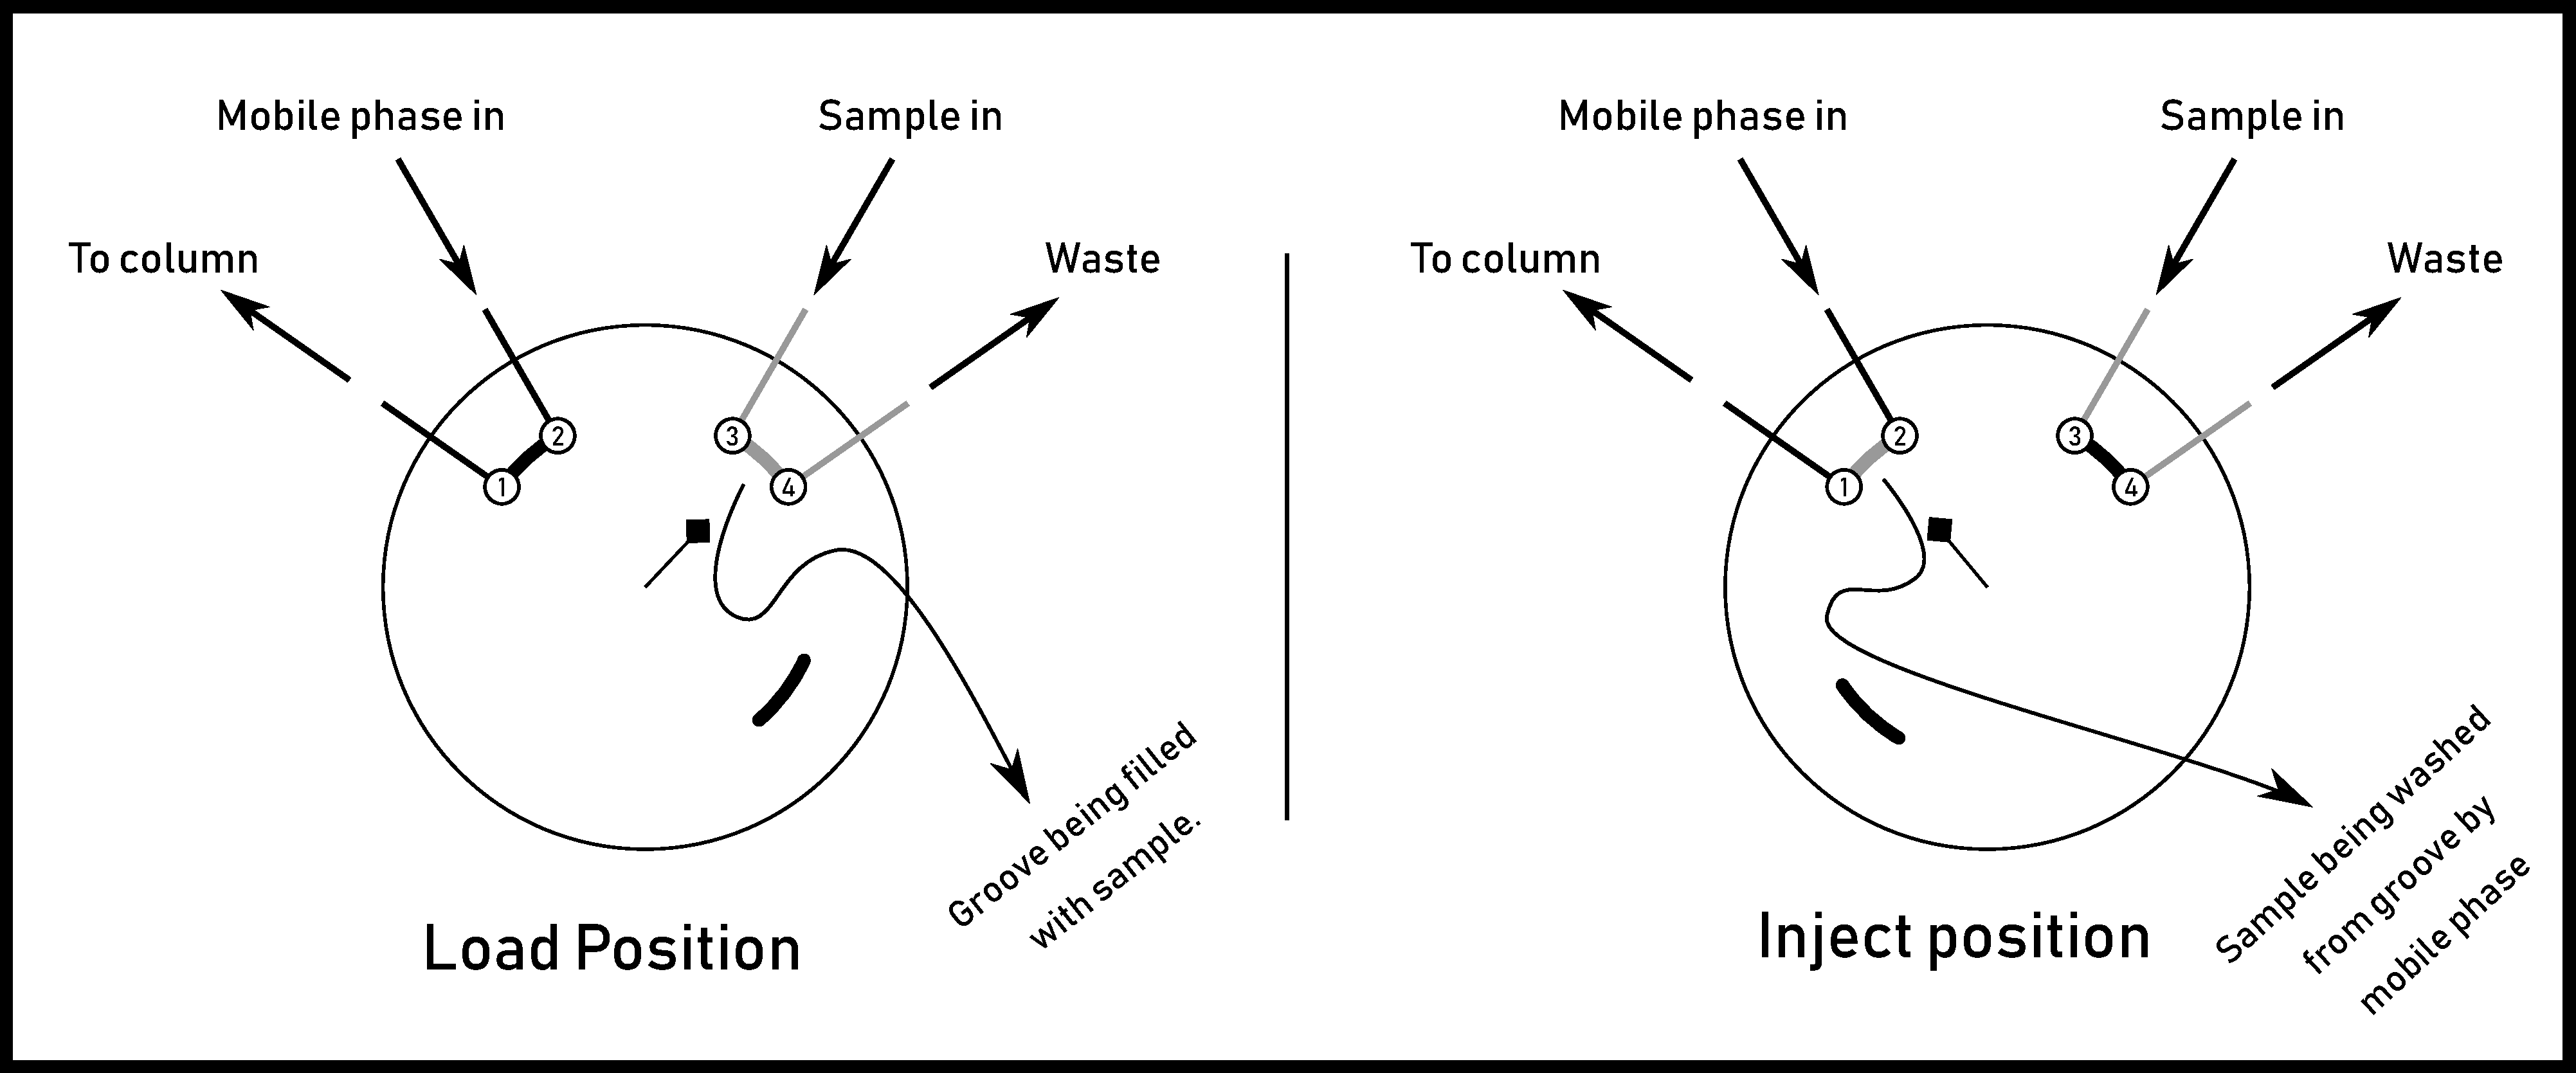
\includegraphics[width=\textwidth]{Figures/SampleValve.pdf}
\decoRule

\caption[Schematic diagram of the injection valve.]{A schematic diagram of the sampling valve. }

\label{fig:samplingvalve}
\end{figure}

The reader might be more familiar with the six-port valve as an injection
system. The benefit of the internal groove injection valve is that it allows a
much smaller volume to be injected. Using this small volume makes it possible to
inject samples without dilution, which simplifies sample preparation. A drawback
of this design is that it is not possible to vary the volume of sample injected.

The sample volume was 5 $\mu$l

The injection valve position was commanded from the controlling PC by electronic
voltage pulses.

\subsection{Column}
\label{sec:SFCColumn}

The separation power of a chromatographic system can be modelled by the equation 

\begin{equation}
R_s = \bigg(\frac{\sqrt{N}}{4}\bigg)  \bigg(\frac{\alpha-1}{\alpha}\bigg)  \bigg(\frac{\bar{k}}{1+\bar{k}}\bigg)
\end{equation}

were, $R_s$ is the \textit{peak resolution}, $N$ is the \textit{number of
plates}, $\alpha$ is the \textit{selectivity}, and $\bar{k}$ is the
\textit{retention factor}.
 
The number of plates $N$ can be increased simply by making the column longer,
at the cost of increasing the time of the run.

The maximum length of the column is determined by the pressure drop available
that will still yield adequate flow. In capillary gas chromatography the
openness of the column and the low viscosity of the gas-phase mobile phase
routinely allows columns 100 metres long at inlet pressures of a few
atmospheres. In HPLC the high viscosity of the mobile phase and the narrow,
tortuous pathways between the small particles of the packing material means that
the columns are typically 100 - 200 mm long, requiring hundreds of atmospheres
of inlet pressure for adequate flow.

The low viscosity of an SFC mobile phase allows operation of much longer
HPLC-type packed columns. This provides a much higher number of plates in the
chromatographic system than HPLC.

The SFC column we used in the SFC×GC system was a set of five HPLC columns (150
mm $\times$ 4.6 mm, 3 $\mu$m particles) (Restek, Pinnacle DB Silica) connected
in series.

The stationary phase in this column is `bare silica', which is usually
considered 'polar'. That means that the packing of the column consists of porous
silica particles with no organic phase covering its surface, and hence one that
will interact strongly with polar molecules. In contrast, the ubiquitous `C18'
stationary phase used in reverse-phase HPLC is 'non-polar'. The particles of
such a stationary phase are coated with octadecyl chains bonded to its surface,
and hence will tend to interact strongly with non-polar molecules. The base
material of the particles is usually silica, but that is only because
manufacturing uniform particles of a given size from silica is a mature
technology and not because silica is important to the separation mechanism. (In
fact, some care has to be taken to deactivate the silica so that it does not
contribute to the retention. Such a mixed retention mechanism can lead to peak
tailing.)

\subsection{Stopped-flow}
\label{sec:stopflow}

Among analytical chemists it is the convention that chromatographic runs are
done without interruptions. In our SFC×GC chromatograph we collect fractions of
SFC eluate and separate them by GC. It is possible to collect, store and inject
fractions of SFC eluate while maintaining continuous flow, for example using a
dual storage loop system like the one depicted in Figure
\ref{fig:continuousflow}. But such systems require careful selection of
volumes, fraction collection reservoirs with matching volumes, and an auxiliary
pump.

\begin{figure}
\centering
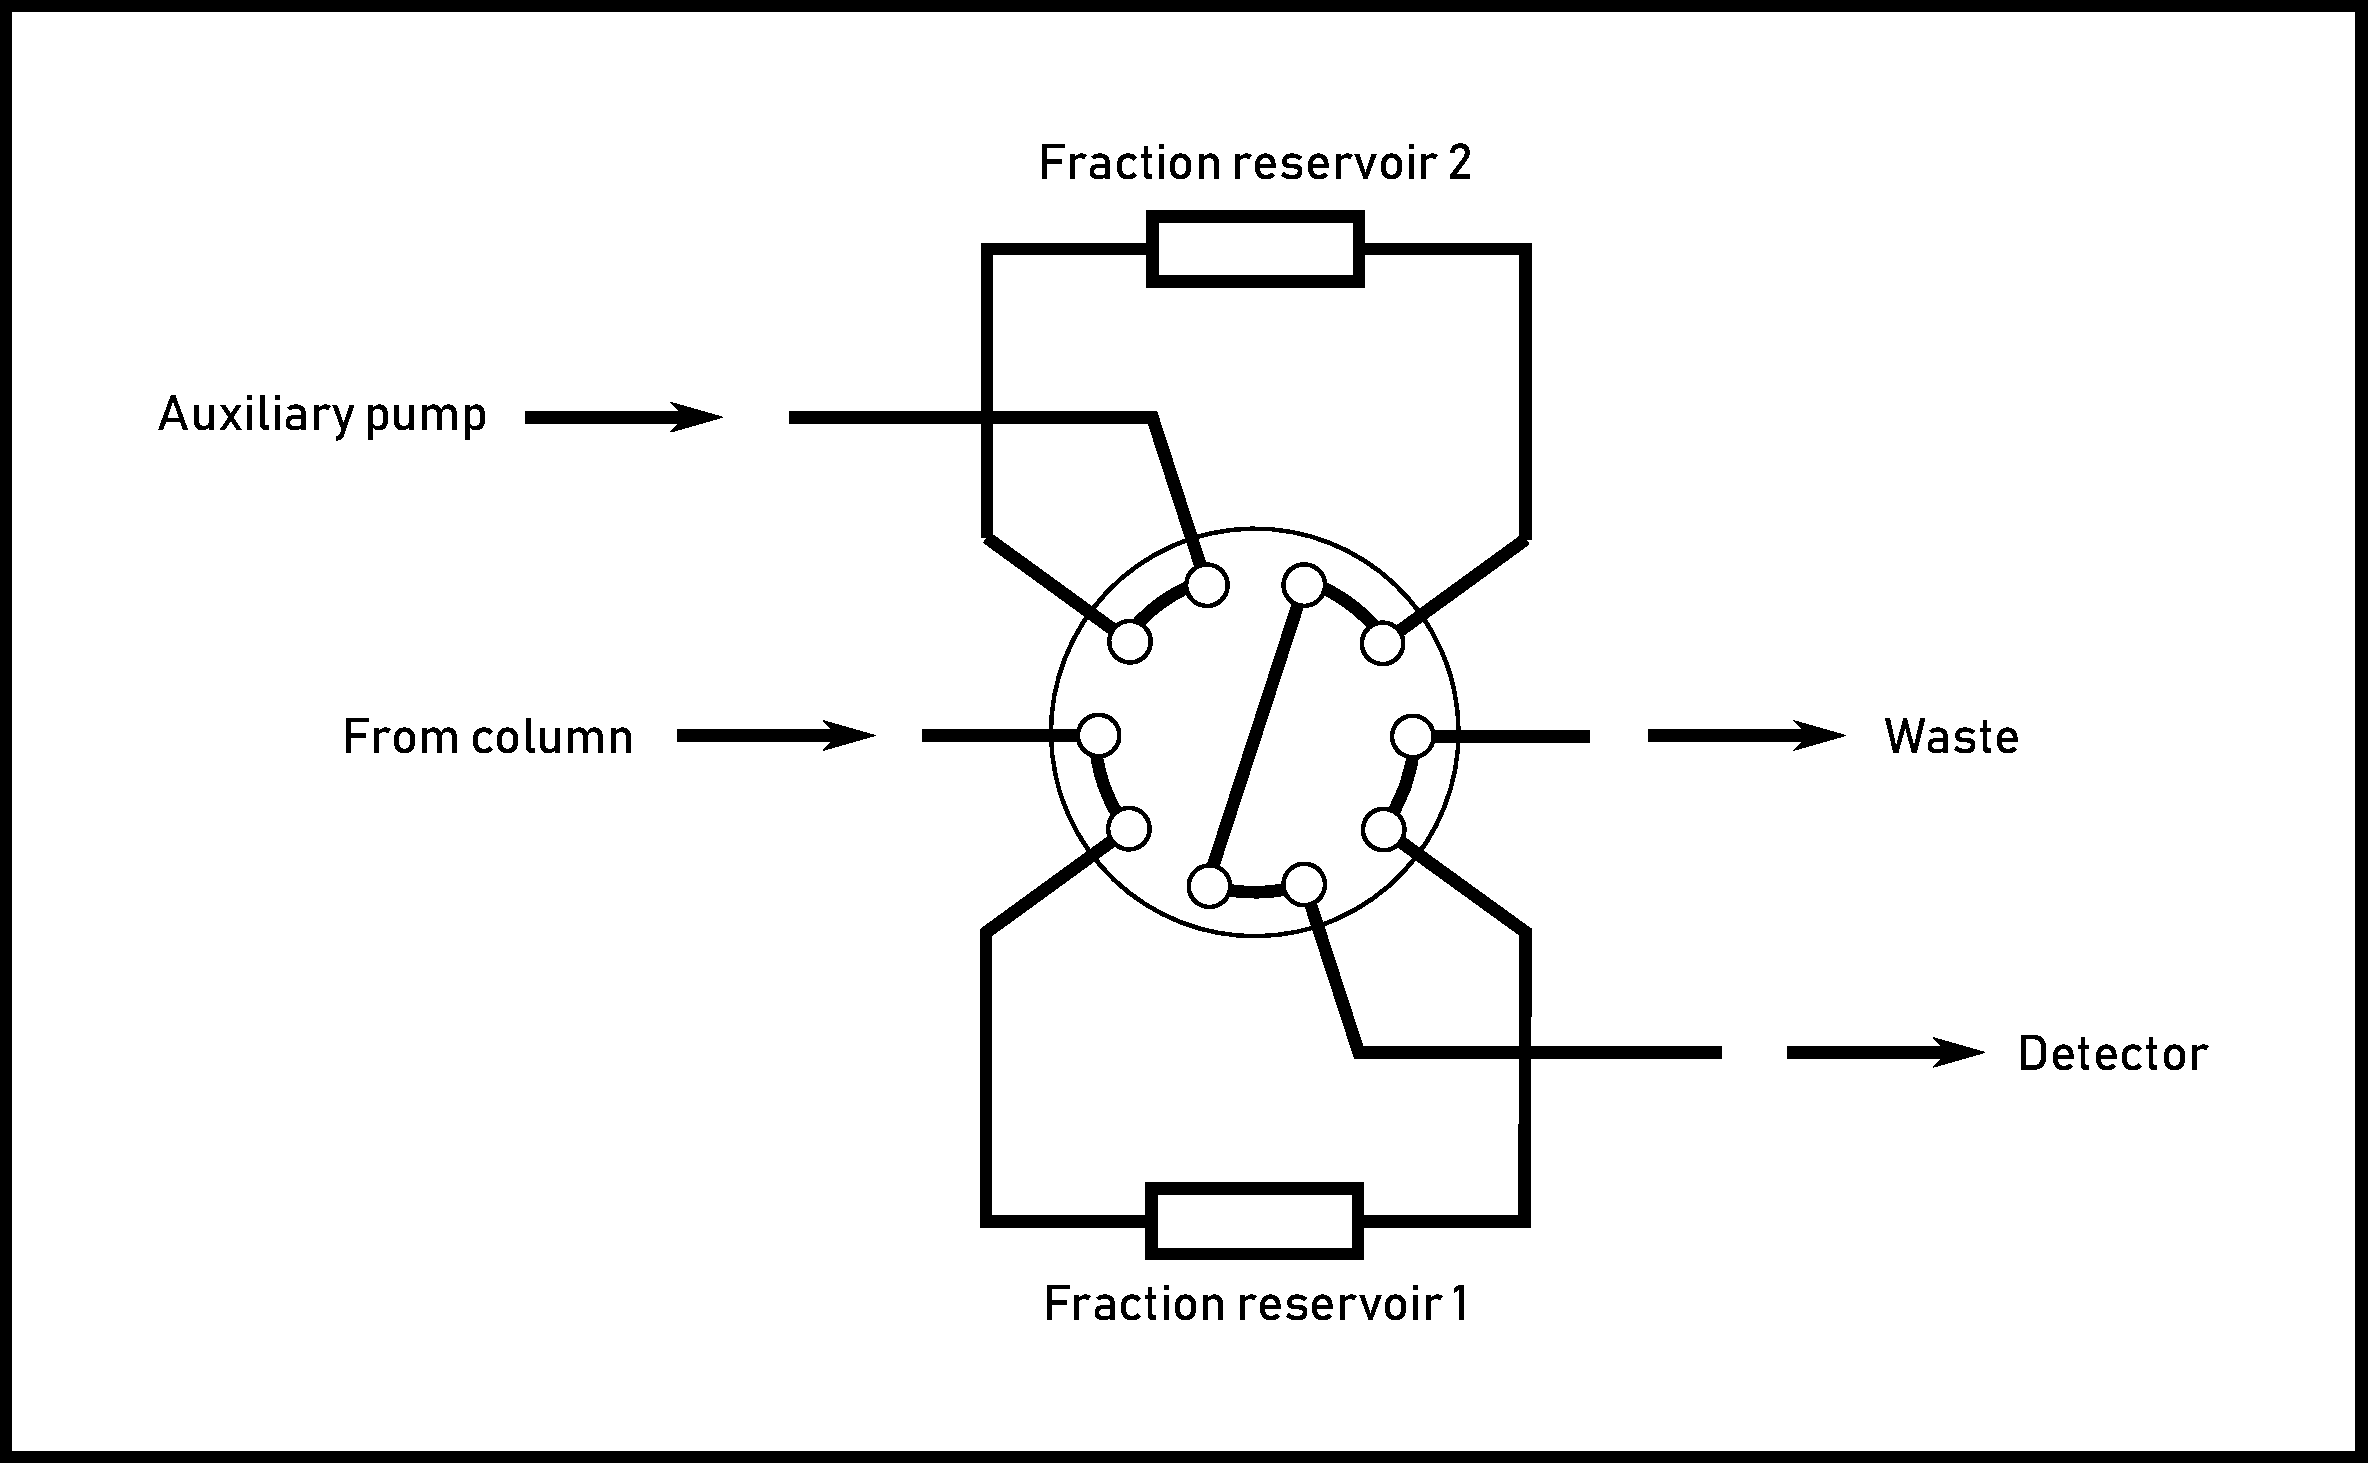
\includegraphics[width=\textwidth]{Figures/ContinuousFlowStopValve.pdf}
\decoRule

\caption[Schematic diagram of a continuous-flow valve.]{A schematic diagram of a
valve configured to allow continuous-flow fraction collection. }

\label{fig:continuousflow}
\end{figure}

Instead of such a system, we opted for a more versatile and simpler stopped-flow
system. In this system a fraction of the SFC eluate is collected, and then the
flow through the column is stopped. While the flow is stopped the collected
fraction is subjected to separation by GC.

In packed columns, "eddy diffusion is always the main cause for peak broadening
at any temperature and at high velocities" \autocite{Gritti2006}. During the
period that the flow is stopped only longitudinal diffusion contributes to peak
broadening, which is small compared to eddy diffusion in dense mobile phases.
Using the simple stopped-flow technique of sample collection will therefore not
have a major effect on the resolution of the \textsuperscript{1}D
chromatography.

The flow in the SFC was stopped by a six-port rotary valve using three of the ports,
directing flow either to a blocked-off port or to the depressurizer, in effect
making it an on-off controller.

\section{Pressure Relief}

No matter the kind of SFC system one uses, at some point the eluate needs to be
depressurized. This can be before or after the detector. If depressurization
happens after the detector, then the details of the mechanism doesn't matter
much, because the information has been obtained and the eluate can be
discarded. If, as in our case, the depressurized eluate needs to still pass the
detector, it is important to not lose the resolution achieved by the column.
This means that the design of the depressurizer requires some care.

The main concern in depressurizer design is premature desolvation of analytes.
This causes \textit{discrimination}, which is the differential treatment of
substances where identical treatments are required. In particular, compounds of
higher molecular weight tend to desolve first from the supercritical fluid, and
might precipitate in the wrong place if the depressurizer is not designed to
prevent it. 

Depressurization can be done either statically or dynamically. In a dynamic
system there is an active element that controls the flow of the eluate in such a
way as to maintain the pressure upstream of the active element of the
controller. Such a device is often called a \textit{back pressure regulator},
and is usually an electro-mechanical device with digital control. They tend to
be complex and expensive.

In static depressurization there is no active pressure control. A simple
\textit{restrictor} is used to limit the flow between the high pressure of the
SFC and the low-pressure outlet. 

Textbooks often discuss different restrictor designs.
\autocite[The book by][provides an example.]{LuquedeCastro1994}. Our preferred
depressurizer was the `integral' or Guthrie design \autocite{Guthrie1986}.
Figure \ref{fig:restrictor} shows the steps in manufacturing the Guthrie
restrictor.

\begin{figure}
\centering
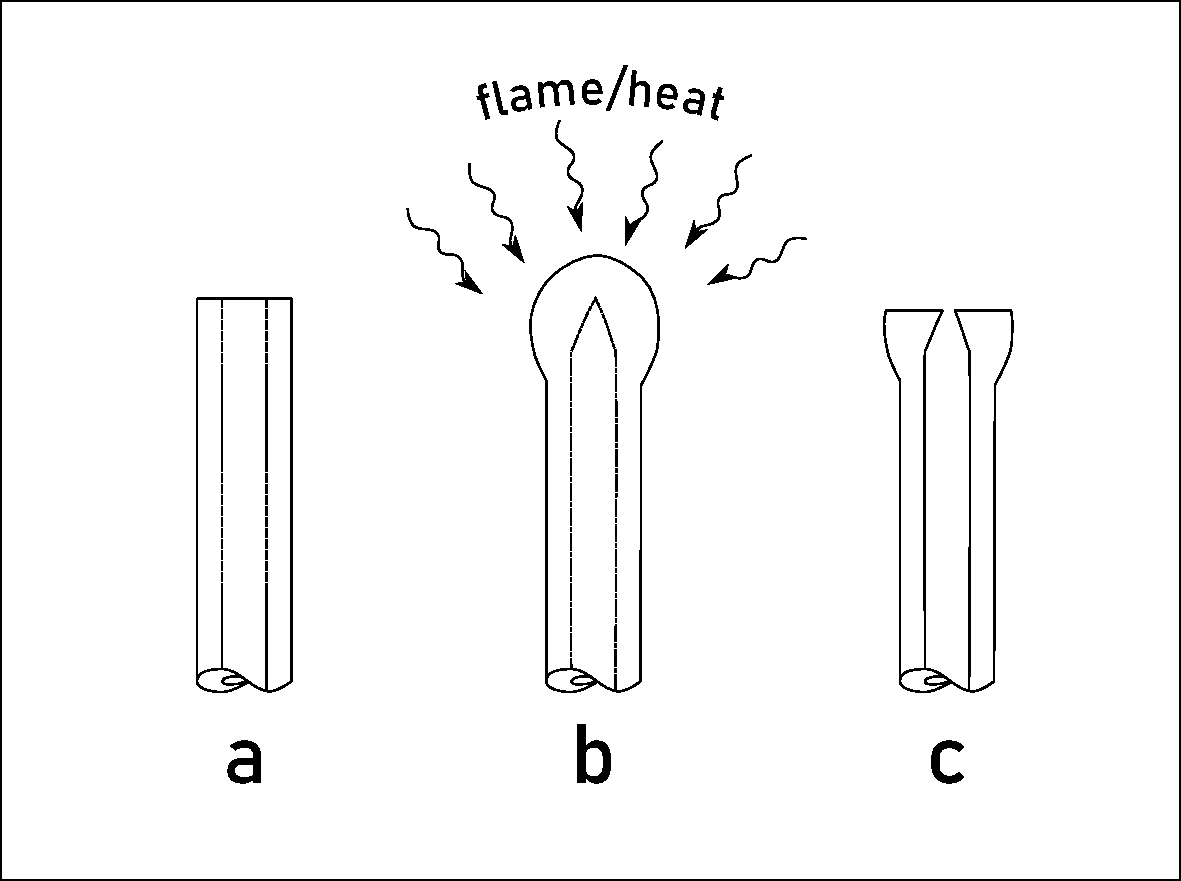
\includegraphics[width=0.5\textwidth]{Figures/Restrictor.pdf}
\decoRule

\caption[A diagram of a integral restrictor.]{The steps of making a Guthrie restrictor. (a) Cut
length of quartz capillary (b) Heat with flame to soften glass and create
internal cone (c) Grind down end to expose orifice of the appropriate size.}

\label{fig:restrictor}
\end{figure}

We found this restrictor robust and fairly simple to manufacture. It was
possible to adjust the flow to a given flow rate. This design of restrictor
should eliminate discrimination, because the decompression takes place in a very
short space.

However, the Guthrie design proved prone to blockage. These blockages could not
be eliminated by incorporating a 0.5 \si{\micro\metre} filter before the restrictor, which
prompted an investigation into the cause of blockages.

To rule out the possibility that it was particles that caused the Guthrie
restrictor to become blocked, we first had to determine the diameter of the
orifice. This proved to be harder than expected: optical microscopy was not able
to give a simple, unambiguous measure of the orifice diameter.

Scanning electron microscopy (SEM) showed that the orifice diameter of a Guthrie
restrictor is about 10 \si{\micro\meter}, as shown in Figure
\ref{fig:restrictororifice} This makes it very unlikely that particles with an
origin in the SFC system blocked the restrictor: even the 3 \si{\micro\meter}
particles from the column packing material should not block this restrictor.

\begin{figure}
\centering
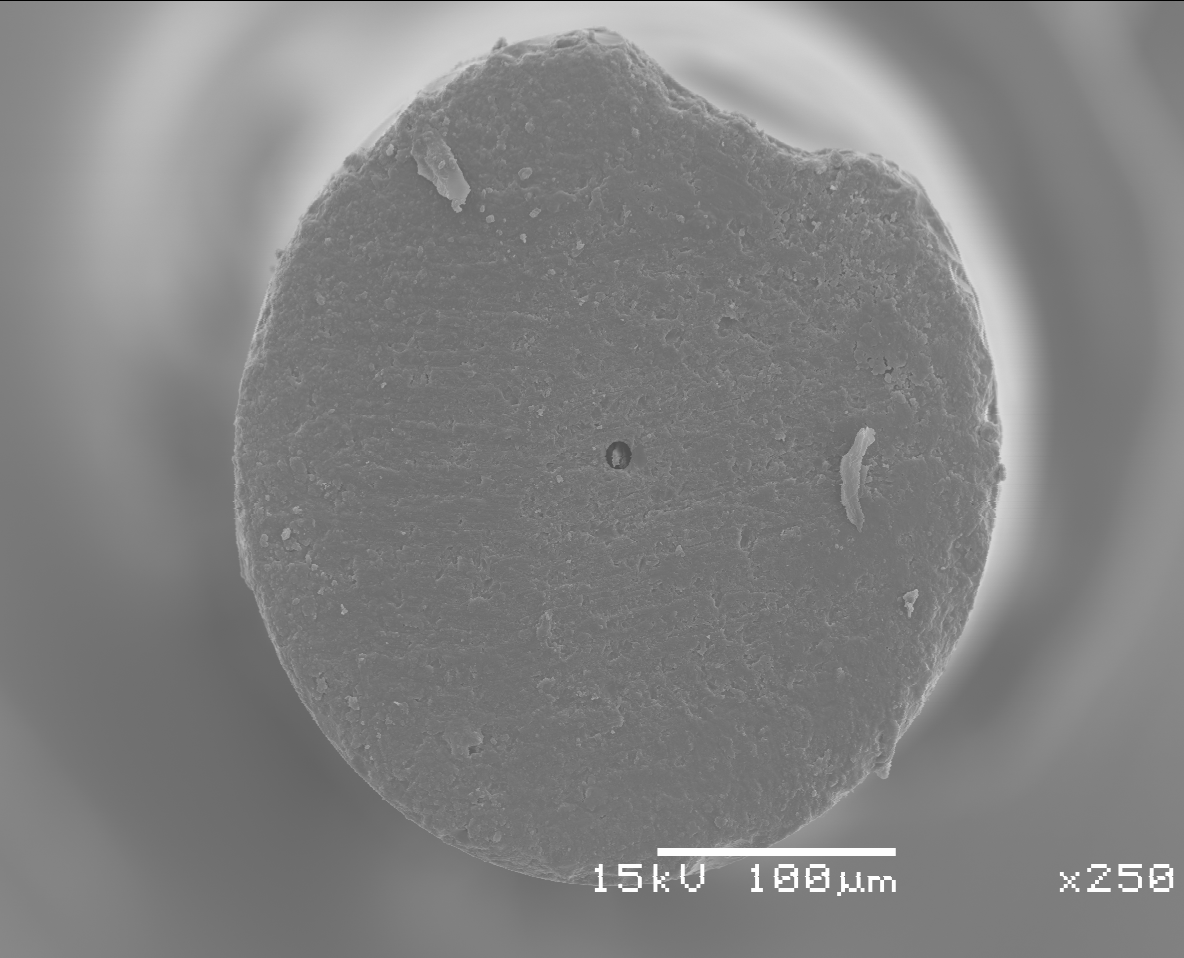
\includegraphics[width=\textwidth]{Figures/sem_h_001.png}
\decoRule

\caption[A electron microscope photo of a restrictor orifice]{An electron
microscope photograph of a restrictor tip, showing the size of the orifice.}

\label{fig:restrictororifice}
\end{figure}

Experience had taught us that the restrictor did not block if the flow was
continuous. It was only when the pressure in the restrictor cycled that
blockages occurred. To eliminate the possibility that it was material from the
stop valve (see Section \ref{sec:stopflow}) that caused the blockages, we cycled
the pressure by switching the pump on and off, allowing the pressure to bleed
off through the restrictor. This way of cycling the pressure did not prevent
blockages.

Examination of blocked restrictors with electron microscopy revealed that the
restrictors became blocked by a soft material. Backscatter SEM mode allows the
energy of X-rays to be measured by energy-dispersive spectrometry, which yields
information about elemental composition. While much care must be taken before
this information can be used for quantitation, it revealed that the deposited
material contains significant quantities of carbon and oxygen, and possibly some
chlorine. This points to the probability that the material blocking the column
is organic in nature, and possibly polymeric. See Figure
\ref{fig:restrictorblockage}.

\begin{figure}
\centering
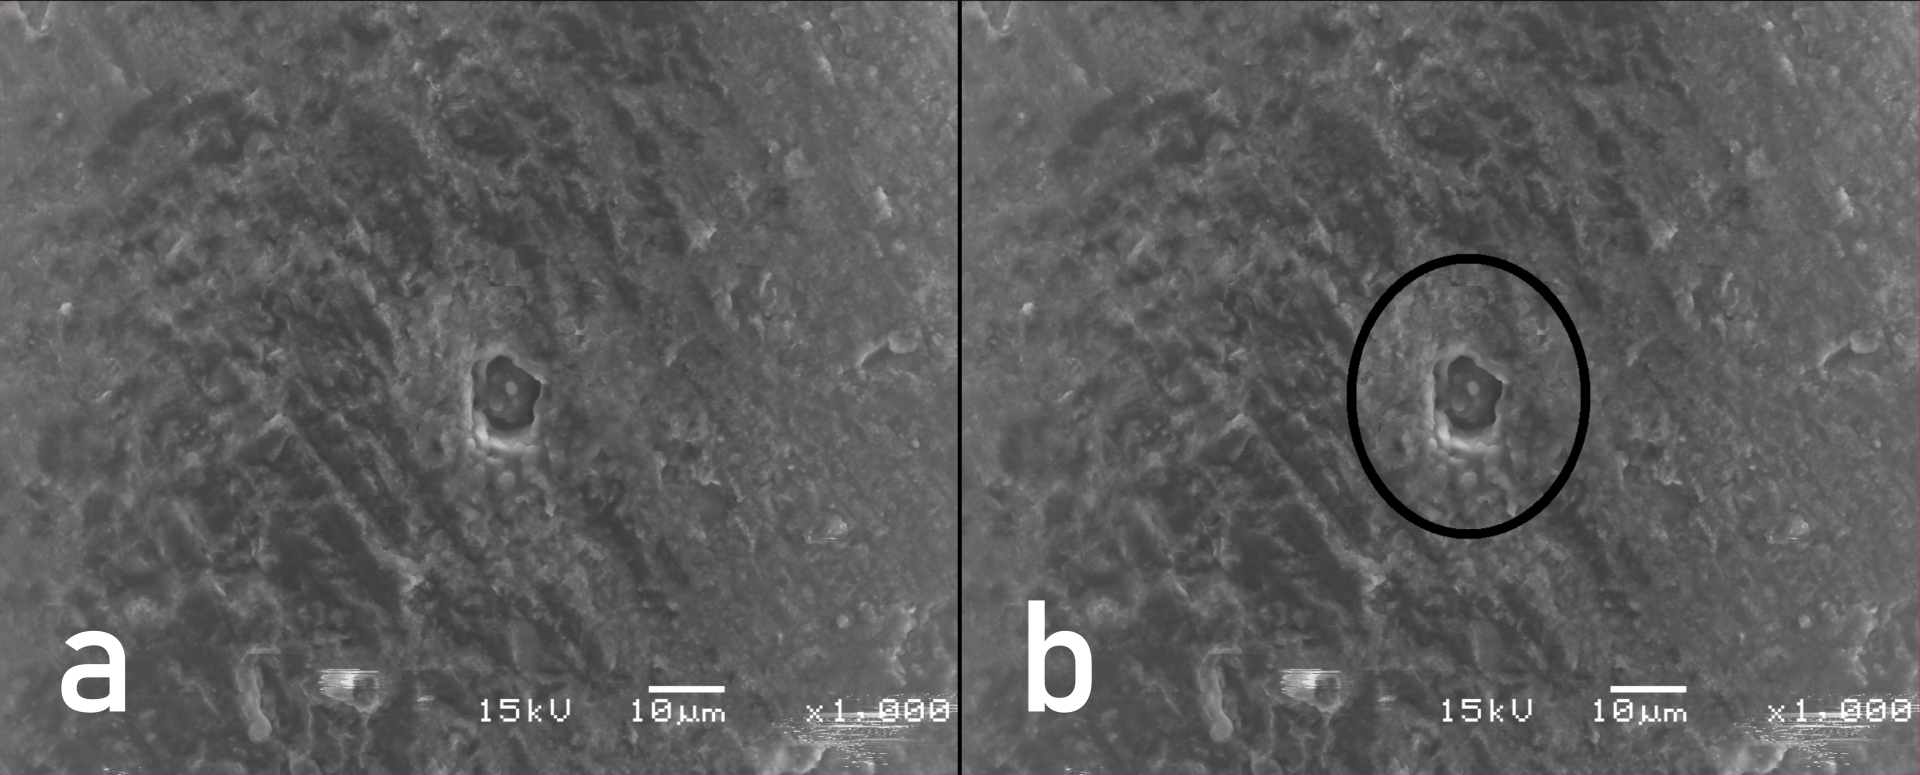
\includegraphics[width=\textwidth]{Figures/Blockage_1920.png}
\decoRule

\caption[A electron microscope photo of a blocked restrictor orifice]{An
electron microscope photograph of a blocked restrictor orifice. (a) Original
image (b) Image with black circle showing estimated original orifice location}

\label{fig:restrictorblockage}
\end{figure}

We could not determine the origin of the material, but it seems likely to be the
column, because cycling the pressure without a column did not cause a blockage.
We eliminated the possibility of blockage by sample material by using a brand
new column. We suspect that the blocking material might be remnants of
surfactants used in the synthesis of the silica gel stationary phase. These
surfactants are leached out of the column packing by the highly diffusive
supercritical fluid mobile phase, and they then precipitate in the restrictor
when the pressure drops and the compounds desolvate. Repetitive pressure cycles
causes a build-up of material which gradually blocks the orifice.

The smallness of the orifice contributes to the plugging problem. With a
diameter of 50 \si{\micro\metre}, a solid sphere that fits in this capillary
will have a volume of .065 \si{\nano\litre}, or 65 \si{\pico\litre}. This means
that nanogram quantities of material can easily block the restrictor.

Being satisfied that an unfortunate combination of restrictor design and column
packing was the likely cause of the blockages, we decided to choose a
different restrictor design. The choice was a simple linear restrictor and
we trusted that heating the end of the restrictor would prevent discrimination.

The linear restrictor was 800 \si{\milli\metre} long and had an internal
diameter of 0.050 \si{\milli\metre}.

\section{Detector}

When SFC was first developed, a capillary column was the usual column, and an
FID was the usual detector. In current use, however, packed columns used with
mobile phase modifiers predominate and flame detectors have lost their place:
the high concentration of modifiers in the mobile phase would swamp the signal
from analytes or saturate the detector. Therefore modern SFC uses
predominantly UV/Vis optical detectors.

In the supercritical fluid chromatograph described in this chapter there was no
dedicated detector: the role of the detector was taken by a gas chromatograph.
This gas chromatograph collected fractions from the SFC, and separated them in
fast chromatographic runs with an FID detector, yielding comprehensive 2D
chromatograms. This chromatograph-as-a-detector is described in Chapter
\ref{Chapter5}.
